\documentclass[10pt]{article}
\usepackage[T1]{fontenc}

% Document Details
\newcommand{\CLASS}{AMATH 585}
\newcommand{\assigmentnum}{Assignment 3}

\usepackage[margin = 1.15in, top = 1.25in, bottom = 1.in]{geometry}

\usepackage{titling}
\setlength{\droptitle}{-6em}   % This is your set screw
\date{}
\renewcommand{\maketitle}{
	\clearpage
	\begingroup  
	\centering
	\LARGE \sffamily\textbf{\CLASS} \Large \assigmentnum\\[.8em]
	\large Tyler Chen\\[1em]
	\endgroup
	\thispagestyle{empty}
}
 % Title Styling
\usepackage{tocloft}
\renewcommand{\cfttoctitlefont}{\Large\sffamily\bfseries}
\renewcommand{\cftsecfont}{\normalfont\sffamily\bfseries}
\renewcommand{\cftsubsecfont}{\normalfont\sffamily}
\renewcommand{\cftsubsubsecfont}{\normalfont\sffamily}

\makeatletter
\let\oldl@section\l@section
\def\l@section#1#2{\oldl@section{#1}{\sffamily\bfseries#2}}

\let\oldl@subsection\l@subsection
\def\l@subsection#1#2{\oldl@subsection{#1}{\sffamily#2}}

\let\oldl@subsubsection\l@subsubsection
\def\l@subsubsection#1#2{\oldl@subsubsection{#1}{\sffamily#2}}
 % General Styling


\usepackage{enumitem}

% Figures
\usepackage{subcaption}

% TikZ and Graphics
\usepackage{tikz, pgfplots}
\pgfplotsset{compat=1.12}
\usetikzlibrary{patterns,arrows}
\usepgfplotslibrary{fillbetween}

\usepackage{pdfpages}
\usepackage{adjustbox}

\usepackage{lscape}
\usepackage{titling}
\usepackage[]{hyperref}


% Header Styling
\usepackage{fancyhdr}
\pagestyle{fancy}
\lhead{\sffamily \CLASS}
\rhead{\sffamily Chen \textbf{\thepage}}
\cfoot{}

% Paragraph Styling
\setlength{\columnsep}{1cm}
\setlength{\parindent}{0pt}
\setlength{\parskip}{5pt}
\renewcommand{\baselinestretch}{1}

% TOC Styling
\usepackage{tocloft}
\iffalse
\renewcommand{\cftsecleader}{\cftdotfill{\cftdotsep}}

\renewcommand\cftchapafterpnum{\vskip6pt}
\renewcommand\cftsecafterpnum{\vskip10pt}
\renewcommand\cftsubsecafterpnum{\vskip6pt}

% Adjust sectional unit title fonts in ToC
\renewcommand{\cftchapfont}{\sffamily}
\renewcommand{\cftsecfont}{\bfseries\sffamily}
\renewcommand{\cftsecnumwidth}{2em}
\renewcommand{\cftsubsecfont}{\sffamily}
\renewcommand{\cfttoctitlefont}{\hfill\bfseries\sffamily\MakeUppercase}
\renewcommand{\cftaftertoctitle}{\hfill}

\renewcommand{\cftchappagefont}{\sffamily}
\renewcommand{\cftsecpagefont}{\bfseries\sffamily}
\renewcommand{\cftsubsecpagefont}{\sffamily}
\fi
 % General Styling
% Code Display Setup
\usepackage{listings,lstautogobble}
\usepackage{lipsum}
\usepackage{courier}
\usepackage{catchfilebetweentags}

\lstset{
	basicstyle=\small\ttfamily,
	breaklines=true, 
	frame = single,
	rangeprefix=,
	rangesuffix=,
	includerangemarker=false,
	autogobble = true
}


\usepackage{algorithmicx}
\usepackage{algpseudocode}

\newcommand{\To}{\textbf{to}~}
\newcommand{\DownTo}{\textbf{downto}~}
\renewcommand{\algorithmicdo}{\hspace{-.2em}\textbf{:}}
 % Code Display Setup
% AMS MATH Styling
\usepackage{amsmath, amssymb}
\newcommand{\qed}{\hfill\(\square\)}

%\newtheorem*{lemma}{Lemma} 
%\newtheorem*{theorem}{Theorem}
%\newtheorem*{definition}{Definition}
%\newtheorem*{prop}{Proposition}
%\renewenvironment{proof}{{\bfseries Proof.}}{}


% mathcal
\newcommand{\cA}{\ensuremath{\mathcal{A}}}
\newcommand{\cB}{\ensuremath{\mathcal{B}}}
\newcommand{\cC}{\ensuremath{\mathcal{C}}}
\newcommand{\cD}{\ensuremath{\mathcal{D}}}
\newcommand{\cE}{\ensuremath{\mathcal{E}}}
\newcommand{\cF}{\ensuremath{\mathcal{F}}}
\newcommand{\cG}{\ensuremath{\mathcal{G}}}
\newcommand{\cH}{\ensuremath{\mathcal{H}}}
\newcommand{\cI}{\ensuremath{\mathcal{I}}}
\newcommand{\cJ}{\ensuremath{\mathcal{J}}}
\newcommand{\cK}{\ensuremath{\mathcal{K}}}
\newcommand{\cL}{\ensuremath{\mathcal{L}}}
\newcommand{\cM}{\ensuremath{\mathcal{M}}}
\newcommand{\cN}{\ensuremath{\mathcal{N}}}
\newcommand{\cO}{\ensuremath{\mathcal{O}}}
\newcommand{\cP}{\ensuremath{\mathcal{P}}}
\newcommand{\cQ}{\ensuremath{\mathcal{Q}}}
\newcommand{\cR}{\ensuremath{\mathcal{R}}}
\newcommand{\cS}{\ensuremath{\mathcal{S}}}
\newcommand{\cT}{\ensuremath{\mathcal{T}}}
\newcommand{\cU}{\ensuremath{\mathcal{U}}}
\newcommand{\cV}{\ensuremath{\mathcal{V}}}
\newcommand{\cW}{\ensuremath{\mathcal{W}}}
\newcommand{\cX}{\ensuremath{\mathcal{X}}}
\newcommand{\cY}{\ensuremath{\mathcal{Y}}}
\newcommand{\cZ}{\ensuremath{\mathcal{Z}}}

% mathbb
\usepackage{bbm}
\newcommand{\bOne}{\ensuremath{\mathbbm{1}}}

\newcommand{\bA}{\ensuremath{\mathbb{A}}}
\newcommand{\bB}{\ensuremath{\mathbb{B}}}
\newcommand{\bC}{\ensuremath{\mathbb{C}}}
\newcommand{\bD}{\ensuremath{\mathbb{D}}}
\newcommand{\bE}{\ensuremath{\mathbb{E}}}
\newcommand{\bF}{\ensuremath{\mathbb{F}}}
\newcommand{\bG}{\ensuremath{\mathbb{G}}}
\newcommand{\bH}{\ensuremath{\mathbb{H}}}
\newcommand{\bI}{\ensuremath{\mathbb{I}}}
\newcommand{\bJ}{\ensuremath{\mathbb{J}}}
\newcommand{\bK}{\ensuremath{\mathbb{K}}}
\newcommand{\bL}{\ensuremath{\mathbb{L}}}
\newcommand{\bM}{\ensuremath{\mathbb{M}}}
\newcommand{\bN}{\ensuremath{\mathbb{N}}}
\newcommand{\bO}{\ensuremath{\mathbb{O}}}
\newcommand{\bP}{\ensuremath{\mathbb{P}}}
\newcommand{\bQ}{\ensuremath{\mathbb{Q}}}
\newcommand{\bR}{\ensuremath{\mathbb{R}}}
\newcommand{\bS}{\ensuremath{\mathbb{S}}}
\newcommand{\bT}{\ensuremath{\mathbb{T}}}
\newcommand{\bU}{\ensuremath{\mathbb{U}}}
\newcommand{\bV}{\ensuremath{\mathbb{V}}}
\newcommand{\bW}{\ensuremath{\mathbb{W}}}
\newcommand{\bX}{\ensuremath{\mathbb{X}}}
\newcommand{\bY}{\ensuremath{\mathbb{Y}}}
\newcommand{\bZ}{\ensuremath{\mathbb{Z}}}

% alternative mathbb
\newcommand{\NN}{\ensuremath{\mathbb{N}}}
\newcommand{\RR}{\ensuremath{\mathbb{R}}}
\newcommand{\CC}{\ensuremath{\mathbb{C}}}
\newcommand{\ZZ}{\ensuremath{\mathbb{Z}}}
\newcommand{\EE}{\ensuremath{\mathbb{E}}}
\newcommand{\PP}{\ensuremath{\mathbb{P}}}
\newcommand{\VV}{\ensuremath{\mathbb{V}}}
\newcommand{\cov}{\ensuremath{\text{Co}\VV}}
% Math Commands

\newcommand{\st}{~\big|~}
\newcommand{\stt}{\text{ st. }}
\newcommand{\ift}{\text{ if }}
\newcommand{\thent}{\text{ then }}
\newcommand{\owt}{\text{ otherwise }}

\newcommand{\norm}[1]{\left\lVert#1\right\rVert}
\newcommand{\snorm}[1]{\lVert#1\rVert}
\newcommand{\ip}[1]{\ensuremath{\left\langle #1 \right\rangle}}
\newcommand{\pp}[3][]{\frac{\partial^{#1}#2}{\partial #3^{#1}}}
\newcommand{\dd}[3][]{\frac{\d^{#1}#2}{\d #3^{#1}}}
\renewcommand{\d}{\ensuremath{\mathrm{d}}}

\newcommand{\indep}{\rotatebox[origin=c]{90}{$\models$}}




 % Math shortcuts
% Problem
\usepackage{floatrow}

\newenvironment{problem}[1][]
{\pagebreak
\noindent\rule{\textwidth}{1pt}\vspace{0.25em}
{\sffamily \textbf{#1}}
\par
}
{\par\vspace{-0.5em}\noindent\rule{\textwidth}{1pt}}

\newenvironment{solution}[1][]
{{\sffamily \textbf{#1}}
\par
}
{}

 % Problem Environment

\newcommand{\note}[1]{\textcolor{red}{\textbf{Note:} #1}}

\hypersetup{
   colorlinks=true,       % false: boxed links; true: colored links
   linkcolor=violet,          % color of internal links (change box color with linkbordercolor)
   citecolor=green,        % color of links to bibliography
   filecolor=magenta,      % color of file links
   urlcolor=cyan           % color of external links
}


\begin{document}
\maketitle



\begin{problem}[Problem 1 (nonlinear pendulum)]
\begin{enumerate}
    \item[(a)] Write a program to solve the boundary value problem for the nonlinear pendulum 
as discussed in the text.  See if you can find yet another solution for the boundary conditions illustrated in Figures 2.4 and 2.5.  

    \item[(b)] Find a numerical solution to this BVP with the same general behavior as seen in Figure 2.5 for the case of a longer time interval, say, \(T = 20\), again with \(\alpha = \beta = 0.7\).  Try larger values of \(T\).  What does \(\max_i \theta_i\) approach as \(T\) is increased?  Note that for large \(T\) this solution exhibits ``boundary layers''.
\end{enumerate}
\end{problem}

\begin{solution}[Solution]

\begin{enumerate}
    \item[(a)] 
        We implement Newton's method to solve the system outlined in the book. 
        \lstinputlisting[linerange=\#<startTeX>-\#<endTeX>]{hw3_1.py}

        Figure~\ref{original} shows the solution converging to the solution found in the book. Figure~\ref{abs} shows a solution not found in the book. Physically this corresponds to sending the pendulum clockwise towards the top, and then having it fall back down. Similar to book Figure 2.5, but in the opposite direction.
        \begin{figure}[H]\centering
            \begin{subfigure}{.45\textwidth}
                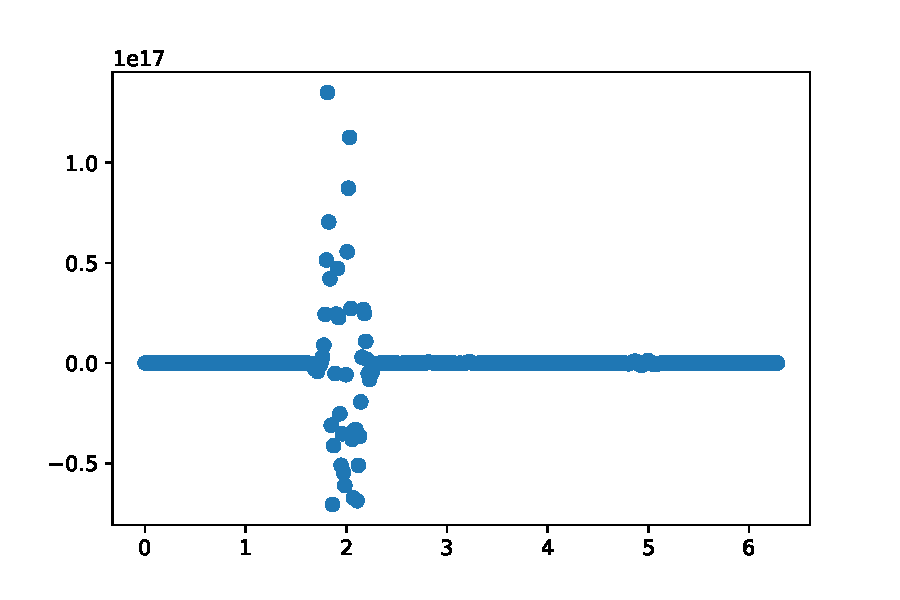
\includegraphics[width=\textwidth]{img/1/original.pdf}
                \caption{\( \theta^{[0]} = 0.7\cos(x) + 0.7\sin(x) \)}
                \label{original}
            \end{subfigure}
            \begin{subfigure}{.45\textwidth}
                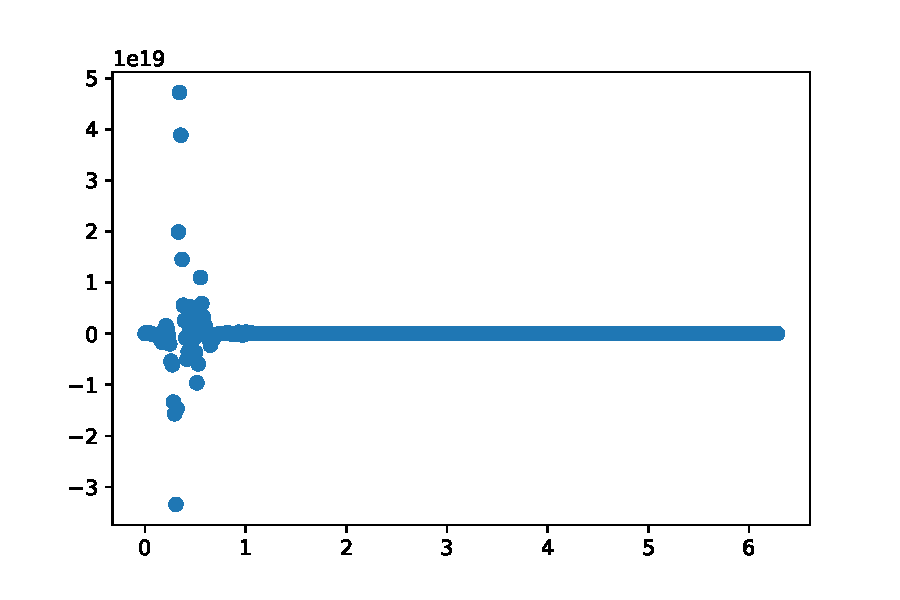
\includegraphics[width=\textwidth]{img/1/abs.pdf}
                \caption{\( \theta^{[0]} = 0.7 + |x-\pi| -\pi \)}
                \label{abs}
            \end{subfigure}
       \end{figure}

    \item[(b)] 
        We now increase \( T \). In order to find a convergent solution we use the previously found convergent solution, scaled (by just using the same indices) from a slightly slower value of \( T \). The results are show in Figure~\ref{p1}.
\begin{figure}[H]\centering
    \foreach \T in {6,14,...,62}{
        \begin{subfigure}{.23\textwidth}
            \includegraphics[width=\textwidth]{img/1/\T.pdf}
            \caption{ \( T = \T \) }
        \end{subfigure}
    }
    \caption{Plots of solution for varying \( T \)}
    \label{p1}
\end{figure}

        The largest value of theta seems to converge to \( \pi \) as seen in Table~\ref{conv}.

        \begin{table}[H]\centering
    \begin{tabular}{|r|l|}\hline
        \( T \) & \( \max_i|\theta_i| \) \\ \hline \hline
        6 & 2.8598081466662055  \\ \hline
        14 & 3.1364877262959778  \\ \hline
        22 & 3.141499073564805 \\ \hline
        30 & 3.1415909367890777 \\ \hline 
        38 & 3.1415926220614177 \\ \hline
        46 & 3.141592653010052 \\ \hline
        54 & 3.1415926535791168 \\ \hline
        62 & 3.1415926535895964 \\ \hline
    \end{tabular}
    \caption{largest value of \( \theta \) for a given \( T \)}
    \label{conv}
\end{table}

        Physically this makes sense. In order for the pendulum to be at \( \theta=0.7 \) at time \( 0 \) and \( T \), with the pendulum moving up and counterclockwise at time \( 0 \), it must go up and almost balance for some time before falling back. If we increase \( T \), the time it spends at the top must be longer and longer. That is, the pendulum will almost be vertical, so that the acceleration is almost zero since it is perpendicular to the force of gravity. 

\end{enumerate}

\end{solution}

\begin{problem}[Problem 2 (Gershgorin's theorem and stability)]
Consider the boundary value problem
\[
- u_{xx} + ( 1 + x^2 ) u = f ,~~0 \leq x \leq 1 ,
\]
\[
u(0) = 0 ,~~u(1) = 0.
\]
On a uniform grid with spacing \(h = 1/(m+1)\), the following set of difference equations
has local truncation error \(O( h^2 )\):
\[
\frac{2 u_i - u_{i+1} - u_{i-1}}{h^2} + (1 + x_i^2 ) u_i = f( x_i ) ,~~i=1, \ldots , m .
\]
\begin{enumerate}
    \item[(a)] Use Gerschgorin's theorem to determine upper and lower bounds on the eigenvalues of the coefficient matrix for this set of difference equations.
    \item[(b)] Show that the \(L_2\)-norm of the {\em global error} is of the same order as the local truncation error.
\end{enumerate}
\end{problem}

\begin{solution}[Solution]

\begin{enumerate}
    \item[(a)] We apply the Gershgorin Theorem for rows. 


        Fix \( i=2,\ldots, m-1 \) and let \( A \) denote the coefficient matrix for this set  of difference equations (note \( A \) depends on \( h \)).

        Then \( A \) is tridiagonal symmetric with,
        \begin{align*}
            a_{ii} = 2/h^2 + (1+x_i^2) && a_{i,i-1} = a_{i,i+1} = -1/h^2
        \end{align*}

        Thus, the Gershorin row disk have radii,
        \begin{align*}
            r_i = \sum_{j\neq i} |a_{ij}| = |-1/h^2|+|-1/h^2| = 2/h^2
        \end{align*}
        
        Since \( A \) is real and symmetric, all eignevalues are real. Denote the part of the \( i \)-th row disk on the real axis by \( D_i \). Then,
        \begin{align*}
            D_i = [a_{ii}-r_i, a_{ii}+r_i] = [(1+x_i^2), 4/h^2+(1+x_i^2)]
        \end{align*}
        
        Given \( h = 1/(m+1) \) and \( x_i = ih \) we have,
        \begin{align*}
            D_i = [1+i^2/(m+1)^2, 4(m+1)^2+1+i^2/(m+1)^2]
        \end{align*}

        We also have,
        \begin{align*}
            r_1 = |1/h^2| && r_m = |1/h^2|
        \end{align*}

        So that,
        \begin{align*}
            D_1 &= [(m+1)^2+1+1/(m+1)^2,3(m+1)^2+1+1/(m+1)^2] 
            \\D_m &= [(m+1)^2+1+m^2(m+1)^2, 3(m+1)^2 +1+m^2/(m+1)^2]
        \end{align*}

        For reasonable values of \( m \) the disks overlap. However, all eigenvalues are contained in \( \cap_i D_i \). That is if \( \lambda \) is an eigenvalue of \( A \), 
        \begin{align*}
            1 + 2^2/(m+1)^2\leq \lambda \leq 4(m+1)^2 + 1 + (m-1)^2/(m+1)^2
        \end{align*}


    \item[(b)] 
        From above it is obvious that all eigenvalues of \( A \) are larger than one. Then, the eigenvalues of \( A^{-1} \) are all less than or equal to one. 

        Thus, this difference method is stable as it is linear, and if \( h \) is sufficiently small, 
        \begin{align*}
            \norm{A^{-1}}_2 = \rho(A^{-1}) < 1
        \end{align*}

        Since the local truncation error is \( \mathcal{O}(h^2) \) and the method is stable, the global error is also \( \mathcal{O}(h^2) \). \qed


\end{enumerate}

\end{solution}

\begin{problem}[Problem 3 (Richardson extrapolation)]
Use your code from problem 6 in assignment 1, or download the code from the
course web page to do the following exercise.  Run the code with \(h = .1\)
($10$ subintervals) and with \(h=.05\) ($20$ subintervals) and apply
Richardson extrapolation to obtain more accurate solution values on the
coarser grid.  Record the \(L_2\)-norm or the \(\infty\)-norm of the error
in the approximation obtained with each \(h\) value and in that obtained
with extrapolation.

Suppose you assume that the coarse grid approximation is piecewise
linear, so that the approximation at the midpoint of each subinterval
is the average of the values at the two endpoints.  Can one use Richardson
extrapolation with the fine grid approximation and these interpolated
values on the coarse grid to obtain a more accurate approximation at
these points?  Explain why or why not?
\end{problem}

\begin{solution}[Solution]

We run the code from assignment one with \( m=10 \) and \( m=20 \) outputting to a \( 2\times 20 \) array. We then apply Richardson extrapolation as,
\lstinputlisting[linerange=\#<startTeX>-\#<endTeX>]{hw3_3.py}

The \( L_2 \) norm of the code with \( m=10 \), \( m=20 \) subsampled down to 10 samples, and the Richardson extrapolation are shown in Table~\ref{richardson}
    \begin{table}[H]\centering
    \begin{tabular}{|r|l|} \hline
        method & \( L_2 \) error \\ \hline \hline
        \( m = 10 \) & 0.0306517881736 \\ \hline
        \( m = 20 \) & 0.0074474900883 \\ \hline
        richardson & 0.000290117131706 \\ \hline
    \end{tabular}
    \caption{\(L_2\) errors using various methods}
    \label{richardson}
\end{table}

Richardson extrapolation works by cancelling the first nonzero coefficient in the error. That is, given an order \( h^k \) approximation, 
\begin{align*}
    \tilde{u}(x,h) = u(x) + a_k(x)h^k + \mathcal{O}(h^{k+1})
\end{align*}
by taking our new approximation as
\begin{align*}
    \dfrac{2^k \tilde{u}(x,h/2) - u(x,h)}{2^k-1} = u(x) + \mathcal{O}(h^{k+1})
\end{align*}
we gain one order of accuracy.

However, this relies on the constants in the expansions for a given \( x \) value to be the same.

Suppose the fine grid spacing is \( h \) and consider a point \( x \) on the finer grid between two points \( x-h \) and \( x+h \) on the coarse grid. The linear interpolation is then,
\begin{align*}
    \dfrac{\tilde{u}(x-h) + \tilde{u}(x+h)}{2} &= \dfrac{u(x-h)+a(x-h)h^2+u(x+h)+a(x+h)h^2}{2} \\
    &= u(x) - \dfrac{h^2}{2} \dfrac{2u(x) - u(x-h) - u(x+h)}{h^2} + h^2\dfrac{a(x-h)+a(x+h)}{2} \\
    &= u(x) - h^2 \dfrac{a(x-h)+a(x+h) - u''(x)}{2}
\end{align*}

Thus, unless \( a(x) = (a(x-h)+a(x+h))/2-u''(x))/2 \) we cannot use richardson extrapolation in the normal way (with \( h, h/2 \) and coefficients \( 4 \) , \( -1 \) and dividing by 3).


\end{solution}

\begin{problem}[Problem 4]
Write down the Jacobian matrix associated with Example 2.2 and the 
nonlinear difference equations (2.106) on p.~49.  Write a code to solve these
difference equations when \(a=0\), \(b=1\), \(\alpha = -1\), \(\beta = 1.5\), and \(\epsilon = 0.01\).
Use an initial guess of the sort suggested in the text.
Try, say, \(h=1/20\), \(h=1/40\), \(h=1/80\), and \(h=1/160\), and turn in a plot of your results.
\end{problem}

\begin{solution}[Solution]

We implement Newton's method to solve \( G(U) = 0 \) where,
\begin{align*}
    G_i(U) = \epsilon \left( \dfrac{U_{i-1}-2U_i+U_{i+1}}{h^2} \right) + U_i \left( \dfrac{U_{i+1}-U_{i-1}}{2h} -1 \right)
\end{align*}

We compute the Jacobian as,
\begin{align*}
    J_{ij}(U) = \begin{cases}
        \epsilon/h^2-U_i/2h & j=i-1 \\
        -2 \epsilon/h^2 + (U_{i+1}-U_{i-1})/2h-1 & j=1 \\
        \epsilon/h^2+U_i/2h & j=i+1 \\
        0 & \text{otherwise}
    \end{cases}
\end{align*}

At each step we solve,
\begin{align*}
    J(U^{[k]}) \delta^{[k]} = - G(U^{[k]})
\end{align*}
starting with initial guess,
\begin{align*}
    U^{[0]} = x - \bar{x} + w_0 \tanh(w_o(x-\bar{x})/2 \epsilon)
\end{align*}
where,
\begin{align*}
    \bar{x} = \dfrac{1}{2}(a+b-\alpha-\beta) &&
    w_0 = \dfrac{1}{2}(a-b+\beta-\alpha)
\end{align*}

We choose the terminating condition \( \norm{\delta}_\infty < 10^{-14} \) or \( k=25 \) iterations. This is implemented in Python
\lstinputlisting[linerange=\#<startTeX>-\#<endTeX>]{hw3_4.py}

We run the code for \( m=10 \times 2^n-1 \) for \( n\in\{1,2,3,4,5,6,7,10\} \). The plots are seen in Figure~\ref{p4}. 
    \begin{figure}[H]\centering
    \foreach \m in {20,40,80,160,320,640,1280,10240}{
        \begin{subfigure}{.23\textwidth}
            \includegraphics[width=\textwidth]{img/4/\m.pdf}
            \caption{ \( m+1 = \m \) }
        \end{subfigure}
    }
    \caption{Plots of solution for varying numbers of mesh points}
    \label{p4}
\end{figure}
\end{solution}

\end{document}
